\chapter{Background Material}

\section{Automatic Content Analysis}
\label{sec:automatic_content_analysis}

\subsection{What is Content Analysis?}
Content analysis is the task of analysing and understanding collections of texts, in other words finding out what a text "is about". The task can be performed by both humans (manual content analysis) and computers (automatic content analysis), and both of the approaches have their advantages and disadvantages.

The concept of manual content analysis is easy. The task is split into first reading and understanding the text, then summarizing the content of the text and/or categorizing it into suitable categories describing the content. As an example, an article about \emph{Ole-Johan Dahl} (the famous Norwegian computer scientist \cite{Olejohandahleng}) would probably be summarized as an article about a famous Norwegian computer scientist and might be categorized under the category \emph{Norwegian computer scientists} if this category is present or the category \emph{computer scientists} if this is present.  
%as an article about authors of children books and Swedish people. 
There are two main disadvantages of manual content analysis which makes it impossible to perform on large collections of texts. The first disadvantage is that the task is time consuming, i.e. it takes time for a human to read and understand an article. The second disadvantage is that manual content analysis requires resources that might be expensive, for instance experts needed for understanding the content of an article if the article is about something beyond common knowledge.

%because some articles needs experts for understanding the content. 
%first has to be read and understood and then we could summarize the content of the text or categorize it under relevant topics.
Automatic content analysis is based on a different approach; instead of reading and understanding the text, the machine looks for predefined properties of the text (in our case known words or phrases) and uses these properties to determine the meaning of the text. This requires some predefined connection between the properties and their associated categories. This approach has disadvantages as well; computers lack commonsense knowledge usually known to ordinary humans, for instance physical description or function of objects. % TODO: Insert reference here.
Color is an example of a physical description computers have problems with determine. Most humans would understand that the phrase \emph{same color as the sun} means yellow, while computers would need specific information about the sun being yellow to conclude the same. 

Another disadvantage with automatic content analysis is dealing with disambiguation. Some words have more than one meaning, and the meaning is usually found from the context or the other words in the sentence. The task of determining the true meaning of a word or sentence is a difficult process which becomes harder if the sentences are complex. 

% TODO: Insert example of complex sentence.

%The easiest way to describe the meaning of the text is to group texts with similar content together, in other word categorize the texts. 

%Some of the advantages with automatic content analysis are that miss


%There are different ways to perform automatic content analysis, our approach is to find the most likely category for texts given as input by first categorizing all articles from Wikipedia. 

%involves using categorization of articles from Wikipedia to determine 

\subsection{Domain of Content Analysis}
Automatic content analysis can be found useful in many different settings, but the 
%There are many areas where content analysis (the task of understanding the content of the text) is useful, but the 
two most dominating areas are advertising and improvement of user experience. The focus for this project is to improve advertising and is therefore the main domain.
%Content analysis is useful for understanding texts, and is often used in two domains; advertising and improving user experience. 

Advertising is the main income of most online companies that provide free services. Many online companies provide their services for free, but make their money on advertisement instead. The alternative to this is to charge users a fee, before they are allowed to use the services. The online market is very competitive and most users expect everything on the Internet to be free. The most common approach is therefore to provide the services for free, but earn money on advertising instead. 

%free services with advertisement is to sell access to to their services, 

%but this is in many cases not possible because the online market is very competitive and many users expect everything on the Internet to be free. 

%difficult in many cases because of how competitive the market is and the expectations of a free Internet. 
%Online advertising is a growing market and is the main income of many online companies. 
%Online companies have two ways of earning money, they could either let the user pay to use the services or earn money on advertisement. Most web pages choose the second option because the market is very competitive and many web users expects the web pages to be free. %A newspaper might loose readers when trying to charge them. 

%Hence the companies have to earn money without charging the user for their services, and in most cases  this leads to advertisement. 
There are different approaches of doing advertisement on web pages. The most common ones are PPC (pay per click) and CPM (cost per mille). CPM is an  advertising technique where the advertiser pays for showing the page to a crowd, while PPC means that an advertisement is shown and the advertiser has to pay for each time a user clicks on the advertisement. Both of the techniques are more valuable for all parts if the advertises are shown to people that are interested and more likely to buy their product. The advertiser has a greater chance of getting customers if the advertisement is shown to the right crowd and the publisher can charge a higher price for the advertisement if the advertiser is more pleased with the result of the advertises.

The main advantage of specified advertisement is that the advertisement can be directed towards users that are more likely to become customers. This means that the advertiser needs to know the users and their interests. Content analysis can be part of building up a profile of the user, since knowing the content of user's text can provide information of the interests of the users. 


\section{Categorization}
Categorization is the process of grouping collections of text into categories, and can be done by both humans or computers. Computer categorization is the technique of teaching a classifier how to decide the category of any input \cite{wiki:categorization}. The idea of this process is to find patterns which makes the machine able to predict the category or class of the input. Such patterns could be similarities between input or decision rules \cite{wiki:classification}. It is desirable to optimize the results of the classifier so that the classifier is as accurate as possible. This can be done by learning the classifier how to behave, either by machine learning where the classifier optimizes itself based on feedback, or by improving the classifier's decision rules.  \\\\
%make the classifier as good as possible,
%Categorization with machine learning can be split into further types; statistical classification which is a \emph{supervised} learning process, and clustering which can be performed as both %an \textit{supervised} and a \emph{supervised} and an \emph{unsupervised} learning process. Supervised learning is a technique where the machine is given a training data set, where the set contains the correct output in addition to the input we want to classify. The classifier uses this data to learn the machine how to behave, also called training the classifier. Unsupervised learning, on the other hand, is the task of trying to find a hidden structure in unlabeled data. The main difference between the two types is that unlabeled data gives no feedback to the classifier, hence the classifier has to assume that it is correctly classified without receiving feedback. It is also possible to have classification processes which are combined of the two, where prior knowledge is given to the classifier. 
%added to the classification process for better results. 
%the data is unlabeled is no feedback sent to the classifier. 
%The classifier will therefore not know if the result is correct, but will continue to classify assuming that the classification performed so far is correct.  
Our problem consists of two categorization problems: 
\begin{enumerate}
\item Categorization of keywords.
\item Categorization of any text.
\end{enumerate}

%the main categorization where any article given as input should be categorized to its most describing category.  

\subsubsection{Categorization of keywords}
The categorization of keywords is done by creating a keyword list based on titles of Wikipedia articles. These keywords have to be categorized to suitable output categories. This categorization could be split into two parts: 

\begin{enumerate}
\item Categorize the keywords to Wikipedia categories represented as category paths  (see figure \ref{fig:keywords_to_categories}). This categorization should be based on the content of the Wikipedia articles of the keywords. Our assumption is that the meaning of a Wikipedia article can be found by looking at the underlying structure of Wikipedia, i.e., the article's categories and the category structure.\begin{figure}[h]
\centering

\includegraphics[width=0.4\textwidth]{Chapters/Background/Keywords_to_categories}
\caption[Categorization of keywords to Wikipedia categories]{Illustration of the categorization of keywords to Wikipedia categories.}
\label{fig:keywords_to_categories}
\end{figure}
\item The complete categorization of the keywords are based on creating a connection between the keywords and categories from IAB's taxonomy (see figure \ref{fig:keywords_categorization_full}). This categorization is based on rules between excerpts of Wikipedia category paths and the output categories. 
\begin{figure}[h]
\centering

\includegraphics[width=0.7\textwidth]{Chapters/Background/Keywords_categorization_full}
\caption[Categorzation process of the keywords]{Illustration of the complete categorization process of the keywords.}
\label{fig:keywords_categorization_full}
\end{figure}
\end{enumerate}
%the categorization by finding rules and apply heuristics. 

%The categorization needed to determine the categories for each article is a statistical classification. Wikipedia's structure is available and this can be used to find the most likely categories. 

\subsubsection{Categorization of any text}
The goal for this project is to be able to categorize any text based on the results from the categorization of the keywords. The classifier for this categorization process needs some rules on how it should classify. Our theory is that occurrences of keywords can determine the content of the text, and multiple keywords categorized to the same category indicate that the text should be categorized to this category. Thus, the classifier needs a way of detecting keywords in the text and a way of determining which category the text belongs to if it contains keywords from different categories. 


%. The main assumption 

%The next classification problem is to classify 
%Our main assumption for content analysis is that articles which contains the same keywords also belong to some of the same categories in Wikipedia. This means that we want create a group of these articles so that similar articles are grouped together. Supervised classification requires, as already mentioned, a training set. The training set of our problem can be defined as articles in Wikipedia since they are already connected to a category within Wikipedia. The task is to create the classifier that use  this information and is able to classify all other articles. 

%does not have a training set because it is almost impossible to create a training set representiing such a large data set. We still have, however,  information about the underlying category structure of the articles in Wikipedia. The goal is therefore to use this information to group similar articles together.
%Our problem is not suitable for supervised machine learning. Trying to solve the problem with supervised classification would lead to some problems that are difficult to solve; it is for instance almost impossible to create a training set to represent such a large data set and it is therefore not possible to create a classification model based on the data. The categorization should therefore be done with unsupervised machine learning, for instance clustering.

%The formal definition of cluster analysis or clustering is the task of grouping similar elements together.Hence the group or cluster should contain elements that share similarities or that are more similar to each other than to the rest of the elements. %This means that elements within a group are more similar to each other than to the rest of the elements, or that the elements within the group have some similarities that make them stand out from the others. 
%Our problem could therefore be defined as a clustering problem, where each cluster or group is the articles which contains some of the same keywords. We want to sort the texts in such a way that texts with similar content are classified to the same cluster and therefore to same category. The problem needs a mapping process so that collections of texts get clustered together within the predefined set of categories. The predefined set of categories will change depending on the purpose of the classification, for instance would advertisement need a different set of categories than categorization of news articles. A proposal to a predefined category set for advertisement is the category set of IAB. 
\section{Wikipedia}
%It has already been mentioned that content analysis needs a keyword list for recognizing words or phrases that are useful for classification. We require that the list is so large that it contains almost all the words that give information of possible categories for the content where the keyword is found.  We have chosen to use Wikipedia to create such a keyword list. 
Wikipedia is a free, online encyclopedia and community that was created by Jimmy Wales in 2001. The encyclopedia is edited by the Wiki-principle, which means that everyone can create and edit articles. To understand the importance of Wikipedia it is worth mentioning that the web page has been ranked as the fifth globally most important web page (New York Times, February 2014), with more than  30 million articles and almost 500 unique users a month. 

Wikipedia contains lots of articles within many subjetcs and is maintained by thousands of people. 
%is a good choice for a base for the keyword list since it contains lots of articles within many subjects and is maintained by thousands of people. 
Hence the idea is to base the list on all the titles in Wikipedia, but the list has to be modified to contain only relevant titles. It is for instance not relevant to have common words in the keyword list which will occur in most articles and not provide any useful information. 
%, like "the" for example, because these will not provide any useful information. 
It is also important to remove or weight down ambiguous words, i.e. words that could confuse the categorization process or apply wrong information. 

One of the main advantages of using Wikipedia is the underlying structure that is already provided. All articles are already categorized which gives information about the content of the article connected to the title. 

%There are many advantages of using Wikipedia, one of them is that all articles are already categorized which gives information about a possible category for each category. This means that the process of mapping between keyword and category  easily can be done by the computer. Another advantage is that it contains articles within various fields and is well maintained.

\subsection{Structure of Wikipedia}
The structure of Wikipedia is web based, where articles with similarities are linked together. Since Wikipedia is language-based, articles only link to other articles within the same language. Wikipedia does also have a category structure, where all articles are classified under at least one category. A category could have articles, but could also have subcategories, where the subcategories have their own articles and subcategories. All the categories form a large category graph where articles are put under the most describing categories, as an example is Ole Johan Dahl \cite{Olejohandahleng} (Norwegian computer scientist) placed under the category \emph{Norwegian computer scientists} instead of the parent category \emph{Computer scientists by nationality} or \emph{Computer Scientists}. 

The category graph is created so there is a link between a category and its subcategories. There is no beginning of the category graph, but here are some categories which have most other categories as their subcategories. These can be though of as beginning categories, also called root categories, and are important when we want to look through all categories in the graph and observe the relationships between them.  Two categories that can be viewed as potential root categories are \emph{Fundamental Categories} or \emph{Main Topic Classifications}. If one of these are chosen as the root category, we can continue through the graph by looking at its subcategories and proceed by looking at each of the subcategory's subcategories an so on.
%An important 
%The easiest way of looking at all categories in the graph is to choose a root category and follow the links to its subcategories and then continue to look 

Figure \ref{fig: subcat_lindgren} is an example of a structure for the category \emph{Astrid Lindgren}, the swedish children's writer. The figure shows a tree structure for the category from the category graph. The figure shows that the category \emph{Astrid Lindgren} has 10 pages directly under the category, and 4 subcategories: \emph{Astrid Lindgrens characters} (9 pages), \emph{Films based on works by Astrid Lindgren} (1 subcategory and 23 pages), \emph{Works by Astrid Lindgren} (2 subcategories and 7 pages) and \emph{Pippi Longstocking} (1 subcategory and 10pages).  This means that there are indirectly 59 pages under the category \emph{Astrid Lindgren} whithout counting pages under the next level of subcategories. 


%is created and how it is fetched from the page for category information.\footnote{\categorytree}

\begin{figure}[H]
\centering
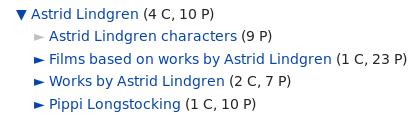
\includegraphics[height=2.5cm]{Chapters/Background/Astrid_Lindgren}
\caption{Subcategories of the category \emph{Astrid Lindgren}. }
\label{fig: subcat_lindgren}
\end{figure}

% HVORFOR IKKE BRUKE WIKIPEDIA SINE KATEGORIER!
Wikipedia articles are already classified under categories, but the set containing all Wikipedia categories cannot be used as a final categorization. The category set in Wikipedia is too large for such usage, where some categories do not provide information of the actual content, and some are too specified. There are also cases where articles are categorized under categories where the combination of the categories does not provide any new information. An example is the article of \emph{Ole Johan Dahl}. Some of the article's categories are showed in figure \ref{fig: olejohandahl_categories}. In this example is the article both placed in the catgory \emph{People from Mandal, Norway} and in the category \emph{Norwegian Computer Scientists}. These categories both provide information about him being Norwegian, so it would be sufficient to put him in the category \emph{Computer Scientists}. The categories are also shown are also quite specific, and it might be desirable with more general categories. 


%of an article where the categories provide the same information, i.e., we already know that he was from Norway since he is in the category \emph{People from Mandal, Norway}, so it would be enough to add that he was a computer scientist instead of specifying that he was a Norwegian computer scientist. 

%categorization between articles and categories cannot be used as a pre-defined category set. 
%Another reason for creating a new independent category set is that Wikipedia categories are not guaranteed to be in the desirable final category set. 

Another reason for creating a new independent category set is that the Wikipedia categories are not guaranteed to be in the desirable final category set. Hence it is essential that the classifier creates a connection from the article and to a category that is know to exist in the set. The classifier should instead be based on the category information provided by Wikipedia. 

%We will therefore need a mapper to a category we know exists. 
%but we cannot use either the categorization from articles to categories nor 
%this categorization is not ideal. It is not possible to use the categorization since a topic might lead
%Another reason why it is not possible to use 
%the category set in Wikipedia as the predefined category set because the category set in Wikipedia is too large. Some categories do not  provide information of the actual content, and some are too specified. There are also cases where articles are categorized under categories where the combination of the categories does not provide any new information. An example is the article of \emph{Ole Johan Dahl}. Some of the article's categories are showed in figure \ref{fig: olejohandahl_categories}. This is an example of an article where the categories provide the same information, i.e., we already know that he was from Norway since he is in the category \emph{People from Mandal, Norway}, so it would be enough to add that he was a computer scientist instead of specifying that he was a Norwegian computer scientist. 

\begin{figure}[H]
\centering
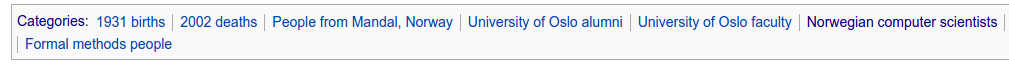
\includegraphics[width=\textwidth]{Dumps/imgs/olejohandahl-categories.png}
\caption[Categories for an Wikipedia article]{Some of the categories for the article of Ole Johan Dahl}
\label{fig: olejohandahl_categories}
\end{figure}

%set is not ideal as a predefined category set for our classifier. 
%There are two main reasons why the categories cannot be based on the categories from Wikipedia. 
%A reason for this is that an article in Wikipedia can be categorized under more than one category and these categories might not be the relevant category set. 
%In many cases are the categories directly subcategories of another category, but in some cases could it be a larger path until a common parent category and the category structure would therefore have to be flatten to make sure it is not classified under conflicting categories. 

%Hva tenkte jeg her? Another reason is that Wikipedia contains


Instead of creating a categorization from the Wikipedia titles and to the most describing categories from Wikipedia's category set, we want to create a connection to a category in a predefined category set. This set of categories should be presented as the desired output and be so simple that it can be understood by the users of the program. The category set should also contain a special category \emph{unknown} for texts where no category is found.

Another requirement for the category set is that the it has to be so well-defined and specific that it conserves as much information as possible about the categorized text. The solution to the problem should also be able to change the predefined category set to another predefined set depending on the texts that are being categorized and the context of the classification.
%that a text is not categorized under conflicting categories, for instance the category "sport" and the category "not sport". We also want the categories to be specific to have more information about the categorized text. 
Hence the best result of the classifier would be found if the set satisfies all of these requirements with the best possible trade off between specialization and generalization. 

\subsection{Accessing Information from Wikipedia}
\label{sec:accessing_information_from_wikipedia}
There are two ways of accessing Wikipedia’s encyclopedic information; the most common way is to enter the webpage and search for the information needed, but it is also possible to download database dumps and access them directly to find information. All Wikipedia articles, images and categories are stored in a database which is accessed whenever a user searches for information online, and the information retrieved from the database is returned to the webpage, for instance in the form of an article. To ensure that all data are safe at all times, files containing the information needed to recover the database is stored and regularly updated \cite{wiki:databasedownload}. This type of backup is called a database dump and is available for anyone interested at \texttt{http://dumps.wikimedia.org/enwiki} \cite{databasedownload}. All Wikipedia files used for this project were downloaded 22nd of January 2015. 
%When a user search for information on the webpage this database is accessed. 
%which are accessed when a user are searching for an article online. 
%A database dump is therefore a backup of the database, and usually stored in the case of some data is lost\footnote{TODO Insert some link here. }. This backup is available for anyone interested at \footnote{TODO:insert link}. 

The files associated with the database dumps contain different information needed, i.e. some files contains all the articles' titles, some contain information about which images belong to which articles and so on. Together they provide all information needed to restore Wikipedia if data is lost. 

%As mentioned, the first step is to find the full path of all articles. Since the Wikipedia articles are placed under categories describing their content, the full path of each article can be found by following the links between categories until an article is found. 

Table \ref{tab:databasedumpfiles} shows the files determined to be relevant for our task and a short description on what they contain. 


%This depends on creating a way to represent the structure of the categories and the articles. 

%and we can therefore define an article's path as the way to reach it from a given category. 
%The first step towards classification of Wiipedia articles is to find all full paths for the articles. There will be more than one way to reach many of the articles. 

%\begin{code}
%[INSERT EXAMPLE]
%\end{code}

%This task depends on different files from Wikipedia and should be split into smaller steps, hence several programs were made to complete the first task. 

%Several files were needed for the task, and the files depended on the language chosen. English is the language with most articles in Wikipedia, hence English were chosen and the 

%The files needed for this task we

\begin{table}[ht]
\renewcommand{\arraystretch}{1.25}
\begin{tabularx}{\textwidth}{l|X}
\textbf{File name} & \textbf{Information contained}\\ \hline
\texttt{enwiki-latest-categorylinks.sql.gz} &  Links between categories, and between categories and articles. \\ \hline
\texttt{enwiki-latest-page.sql.gz} & All pages in Wikipedia, including the type of page (category, article, user) and whether the page is a redirecting page or not\\ \hline
\texttt{enwiki-latest-page\_props.sql.gz} & The properties of each page, including if the category is a hidden category or if the page a disambiguation page. \\ \hline
\texttt{enwiki-latest-redirect.sql.gz} & Redirects from Wikipedia pages and to other Wikpediapages. \\ \hline
\texttt{enwiki-latest-category.sql.gz} & Properties of all categories. \\ \hline
\texttt{enwiki-latest-langlinks.sql.gz} & Links from English Wikipedia pages to the same page in other languages.
\end{tabularx}
\\[10pt]
\caption[Relevant files from English Wikipedia database dump]{The relevant files from the English Wikipedia database dump and a short description of what they contain}
\label{tab:databasedumpfiles}
\end{table}

\section{Interactive Advertising Bureau (IAB)}
The predefined category set should be well-defined and fit for the purposes of the task. Since the focus of this project is improving advertising, the predefined category set should be a category set useful for advertising. 


%The machine learning need a predefined set of categories for the clustering. It is already mentioned that Wikipedia has articles stored under categories and that the categories form a tree or graph structure. The problem is that there are too many categories that are not relevant for our categorization.

%The problem is therefore using IAB's categories for the clustering. 

IAB is a business organization that develops, researches and maintains industry standards for the online advertising industry. The organization works for coalescing and maintaining standards and practices in online advertising. IAB also does research and share knowledge on the advertisement and is responsible for distributing 86 \% of all the online advertisement in the US \cite{IABabout}.

IAB has a predefined set of categories that are developed as part of the Quality Assurance Guidelines Taxonomy. This set is well-defined for advertising, and is split into two layers also called tiers. The layers are created for varying the grade of speciality. The first tier is a general or broad level where the categories are quite general, with a total of 23 categories, including \emph{Business} or \emph{Food \& Drinks}. The second tier is a deepening level containing 371 subcategories of the categories of the first tiers.
%, where the categories are subcategories of a category in the first tier.
Figure \ref{fig:IAB} shows the taxonomy of IAB as defined on their web page where the first tier is all the category names written in white (eg. \emph{Food \& Drinks}) and the second tier is followed under the first tier (eg. \emph{American Cuisine}). This taxonomy is written as a category set that is used for our project. Table \ref{tab:taxonomyascategories} is an example of how parts of the taxonomy for \emph{Food \& Drinks} and \emph{Hobbies \& Interests} is written as a category set, where the second tier is placed under the first tier. This means that an article mapping to \emph{Chinese Cuisine} maps to the category \emph{Food \& Drinks/Chinese Cuisine}.

\begin{table}[h]
\centering
\begin{tabular}{l|l}
%\textbf{Tier 1} & \textbf{Tier 2} \\ \hline
\textbf{Food \& Drinks} & \textbf{Hobbies \& Interests} \\ \hline
American cuisine & Art/Technology\\
Barbecues \& Grilling & Arts \& Crafts\\
Cajun/Creole & Beadwork \\
Chinese Cuisine & Birdwatching\\
Cocktails/Beer & Board Games/Puzzles\\
Coffee/Tea & Candle \& Soap Making\\
Cuisine-Specific & Card Games\\
Desserts \& Baking & Chess \\
... & ...
\end{tabular}
\caption{Example of how the IAB taxonomy changed to a category set}
\label{tab:taxonomyascategories}
\end{table}




%The category set from IAB's taxonomy is a well-defined category set to use of our clustering problem.  




% I stedet kan vi bruke Wikipedia-kategoriene for en sjekk for å se om v har kategoriesert rett?
%
\begin{figure}[t]
%\centering
\begin{subfigure}{\textwidth}
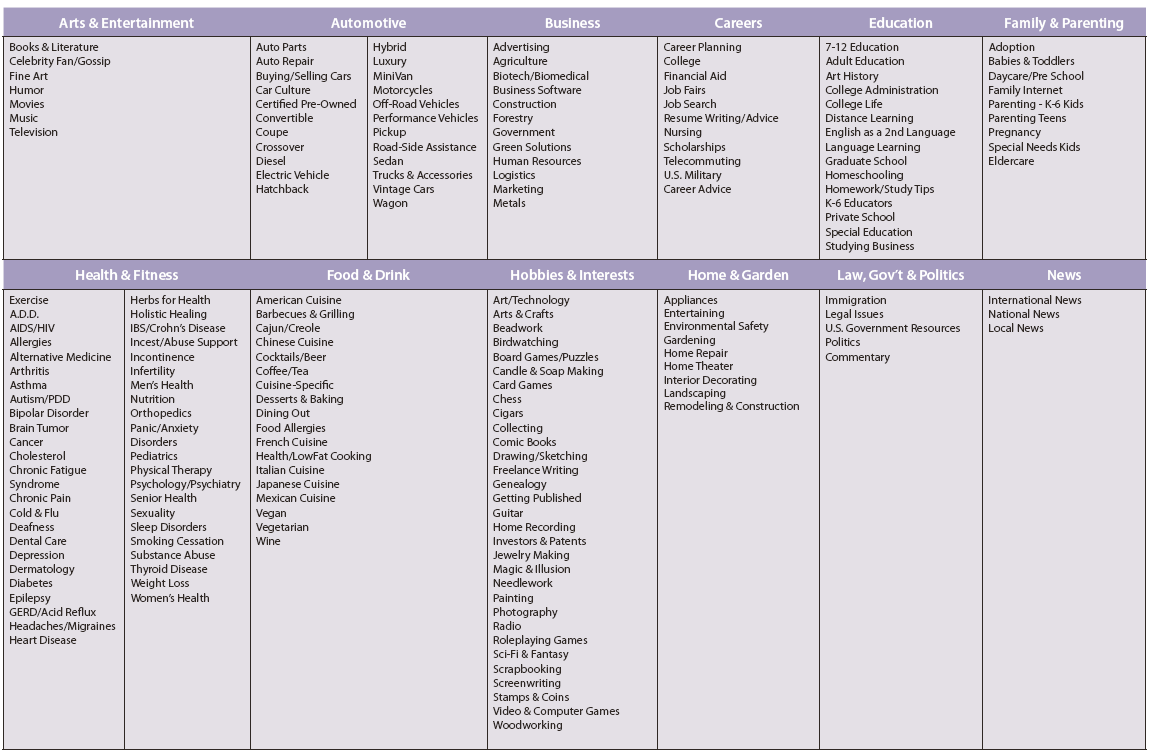
\includegraphics[width=\textwidth]{Chapters/Background/Taxonomy-1.png}
%\caption{Categories of the IAB Taxonomy}
%\label{fig:IAB1}
%\end{figure}
\end{subfigure}
\begin{subfigure}{\textwidth}
%\begin{figure}[H]
\centering
%\newline
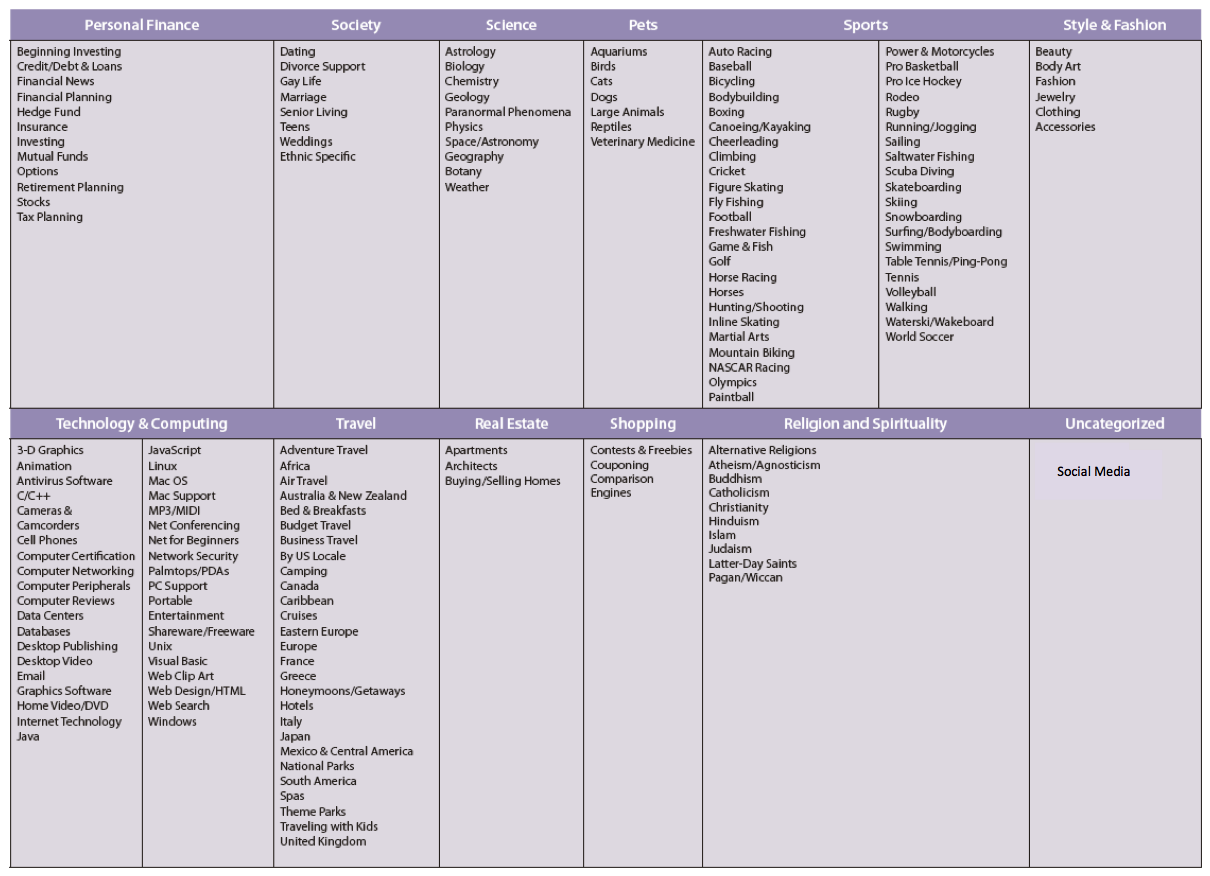
\includegraphics[width=\textwidth]{Chapters/Background/Taxonomy-2.png}
\end{subfigure}
\caption{Categories of the IAB Taxonomy}
\label{fig:IAB}
%\label{fig:IAB-categories}
\end{figure}
%Figure \ref{fig:IAB-categories} 


%When categorizing a collection of texts, similar texts will be in the same cluster and therefore in the same category. This can be used to determine the content of the text. 

%The content analysis need a list of keyword to look for in texts. 



%
\subsection{Advantages with Automatic Content Analysis}
The main advantage with automatic content analysis is time, computers work ve

\subsection{Issues}
% Main issues: 
% predefined set
% predefined keyword list
% Common knowledge -> how to represent this
Even though there are many advantages of using automatic content analysis, there are also some issues with categorization that need to be dealt with for optimal results. 
%There are some issues with automatic content analysis that are important to handle. 
The first is that the computer can only think what its learnt to think, hence cannot define its own categories but needs a predefined set of possible categories. It is a lot easier to ask the computer "Is the article about a computer scientist" than to let the computer find this possibility itself. The other issue is to decide what words are important and useful for deciding the categories of a text. 

%The computer content analysis is an automatic categorization process, where we want to find words that help us define the categories of the text. 
The first issue can be solved by defining a set of categories that we want to categorize text into. This set of categories should be presented as the desired output and be so simple that it can be understood by the users of the program. The category set should also contain a special category \textit{unknown} for texts where no category is found.
%There are some requirements that need to be met for our set; the set has to be so large that all relevant texts can be placed under at least one category, and it has to be so general that similar texts have a high probability of being categorized together. The category set should also contain a special category \textit{unknown} for texts where no category is found. 
%Another requirement for the category set is that the it has to be so well-defined and specific that it conserves as much information as possible about the categorized text. The solution to the problem should also be able to change the pre-defined category set to another pre-defined set depending on the texts that are being categorized and the context of the classification.
%that a text is not categorized under conflicting categories, for instance the category "sport" and the category "not sport". We also want the categories to be specific to have more information about the categorized text. 
%Hence the best result of the classifier would be found if the set satisfies all of these requirements with the best possible trade off between specialization and generalization. 

Feature selection is an important part of classification, and is defined as the process of selecting relevant features which will be used for the classification. It is natural to use words or phrases as features in classification of text, hence feature selection is the issue of deciding the words or phrases that are useful for categorization. These should be collected in a predefined list of keywords where our task is to create a mapping from the keywords to one or more categories that are describing for the text. The category mapping is a way of saying that a text is more likely to belong to the keyword's category if the word is present in the text. If an article mentions "Pippi Langstrømpe" (the main character in many of Astrid Lindgren's children books), the probability for the article to be about Astrid Lindgren or belong to the category "Swedish children's writers" should be larger than if the articles does not mention the name. The keyword "Pippi Langstrømpe" should therefore have some mapping to this category. 


%Input noe om wikipedia og mediawiki

\input{Chapters/Background/Challenges}

\begin{comment}
About content analysis
 - What is content analysis?
    * Automatic content analysis
 - Advantages with Automatic Content Analysis
 - Issues
    * Difficulties
 - Domain of Content Analysis 
 
Categorization 
 - What is categorization: manual vs automatic
 - Unsupervised categorization, clustering, rule-based (heuristic)
 
 Wikipedia 
  - What is Wikipedia?
 
 
 IAB 

\end{comment}